\documentclass[a4paper,10pt]{article}
\usepackage[english]{babel}
\usepackage[utf8]{inputenc}
\usepackage{graphicx}
\usepackage{amsmath,amssymb}
\usepackage{hyperref, url}
\usepackage{listings}
\usepackage[multiple]{footmisc}
\usepackage[english]{babel}
\usepackage{float}
\parindent 0mm
\parskip 3mm

% add your name and student number in parenthesis
\title{ICS-E4020: Week 1 - Median Filtering}
\author{Néstor Castillo García (472081)\\ 
       {\tt nestor.castillogarcia@aalto.fi}}
\begin{document}

\maketitle

\section{Median Filtering}

\subsection{Description}

A median filter was implmented for png images such that for each colour component, the value of each pixel is the median of all pixel values within a sliding window of dimensions (2k+1) x (2k+1).

\subsection{Implementation}
The implmentation was tested using arrays and vectors, the performance was equivalent in both cases. The median function uses the nth\_element function in the c++ algorithm library. The complexity of the median function is O(n). The algorithm calculates the median for every pixel in the image. Only mf1 and mf2 exercises were implemented.


\subsection{Hardware}
The computers had the following specifications: Intel Xeon E3-1230v2, 4 cores, 8 thread, 3,3 GHz, RAM: 16 GB, GPU: Nvidia K2000.

\pagebreak
\subsection{Benchmark}

In figure 1 can be seen that an increase in the window size represents an exponential growth in the processing time. It can be seen that for one thread and a window size of k = 10 the processing time is slightly smaller than four seconds. In addition the time drops dramatically when using more threads.

\begin{figure}[H]
\centering
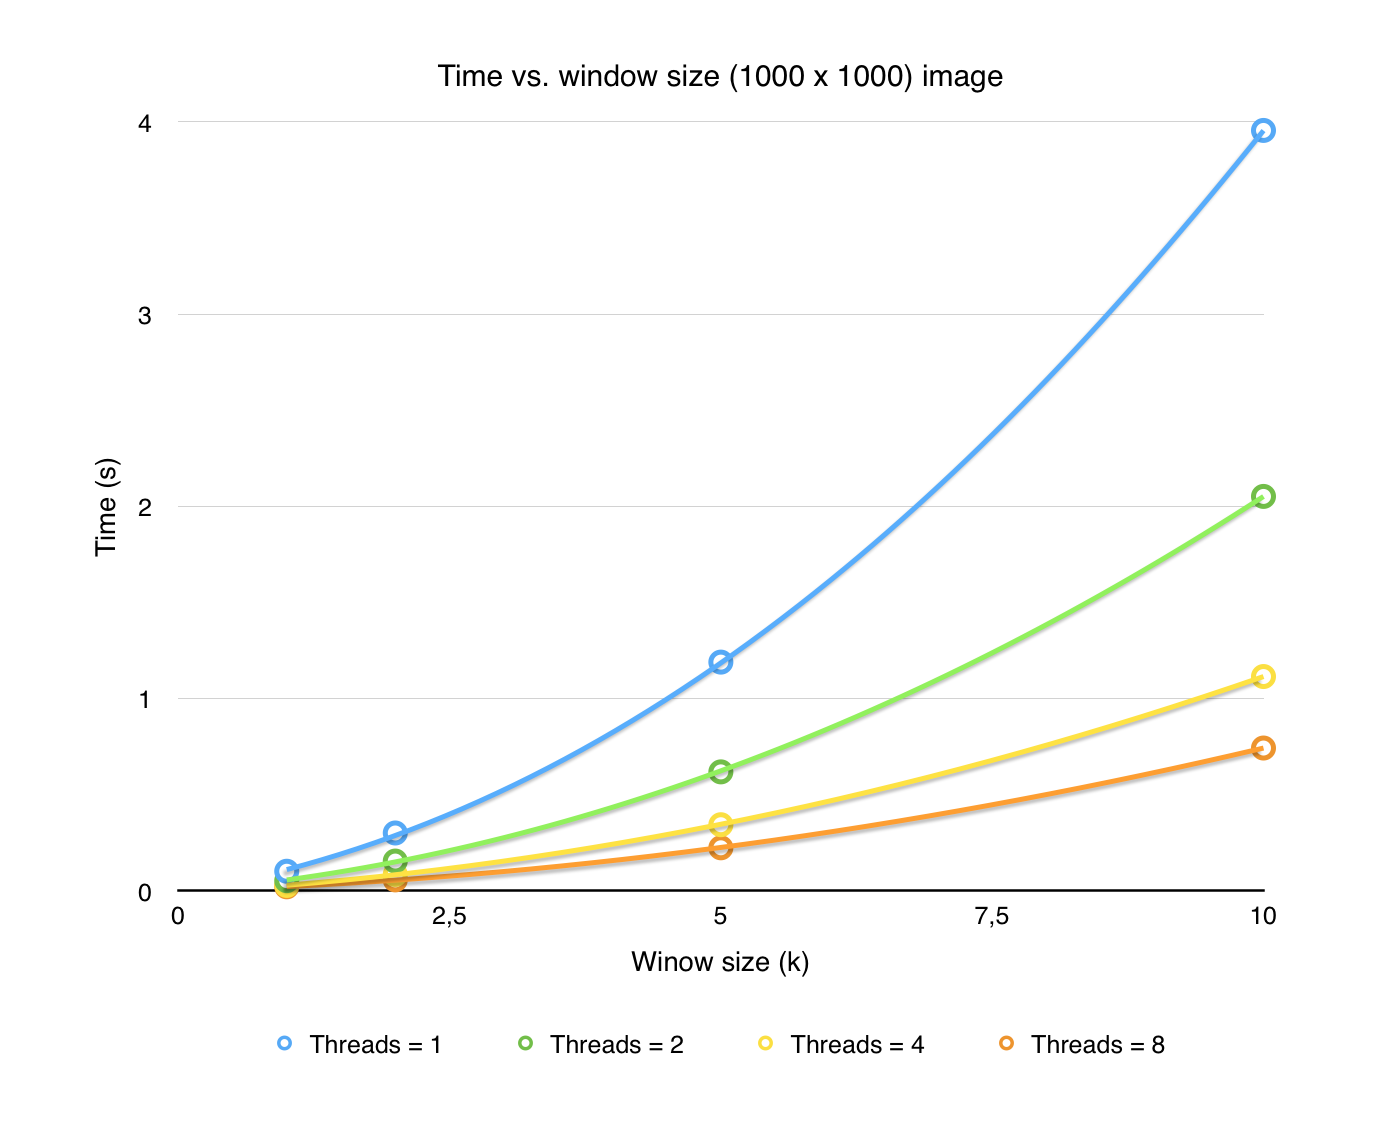
\includegraphics[width=1\textwidth]{figures/w1_timeVsSize}
\caption{Processing time vs window size in a 1000 x 1000 image}
\label{fig:pca_type}
\end{figure}

In figure 2, the time was standarised dividing it by the greatest value to appreciate its decrease in percentage when compared to a single thread implementation. The time used was the average of the computing time for window sizes k = 1,2,5 and 10 for 1,2,4 and eight threads. It can be seen that the time for two threads is half of the time of a single one and the time for four threads is a quarter of a single thread. However, for eight threads the results are slightly better than four threads but not an octave of the single threaded processing time. This is because the computer has only four physical cores and the eight threads are achived with hyper-threading.

\begin{figure}[H]
\centering
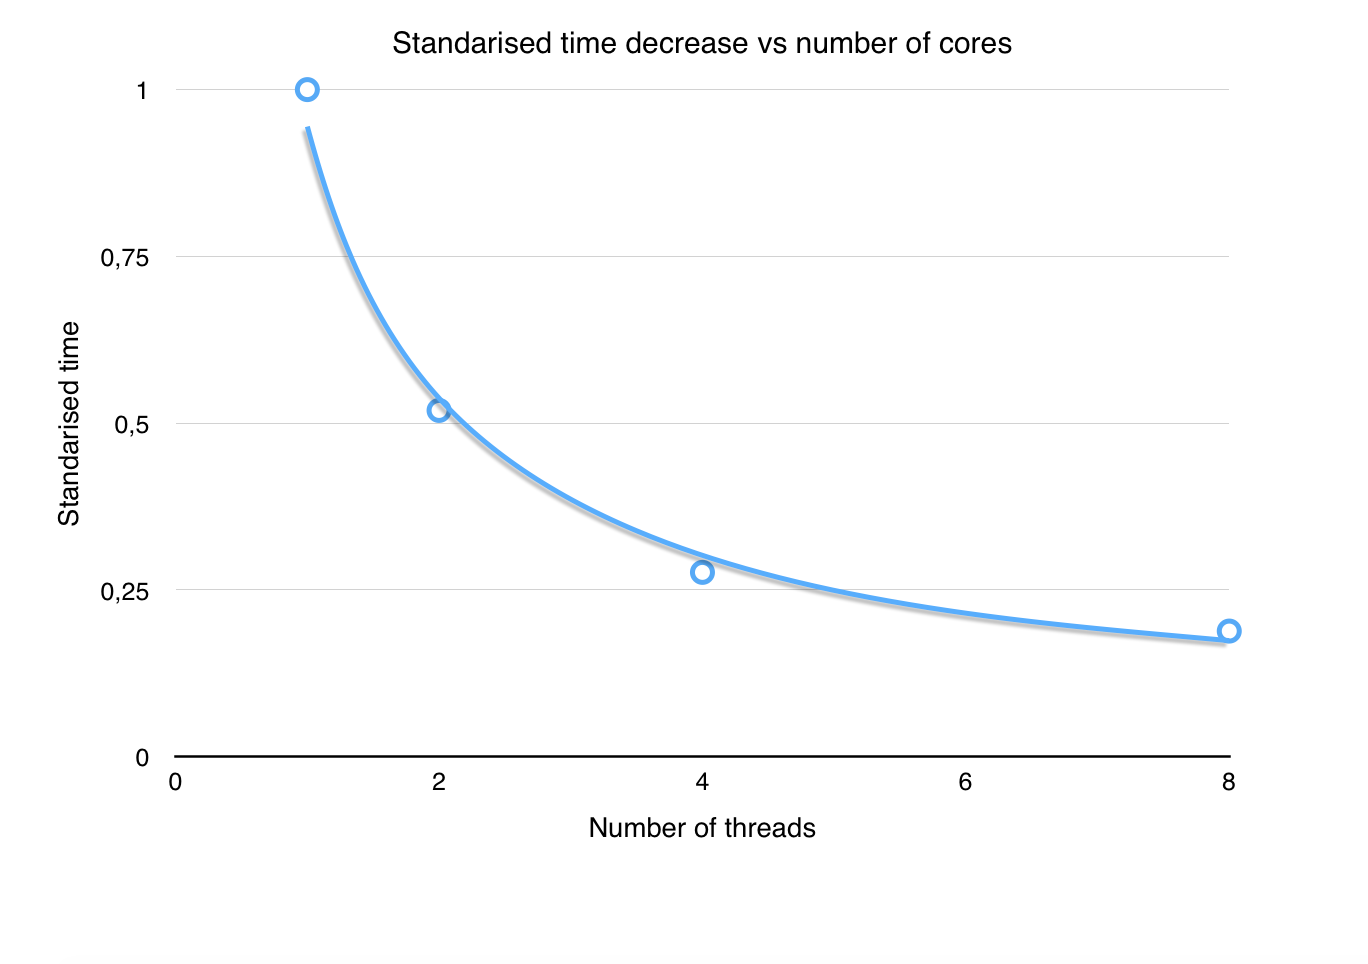
\includegraphics[width=1\textwidth]{figures/w1_timeVsCores}
\caption{Time decres vs increse in threads}
\label{fig:pca_type}
\end{figure}

The following table contains the benchmark results for different image sizes and number of threads. 

\begin{table}[h]
\begin{tabular}{|l|l|l|l|l|l|l|}
\hline
\textbf{img. width} & \textbf{img. height} & \textbf{k} & \textbf{Threads = 1} & \textbf{Threads = 2} & \textbf{Threads = 4} & \textbf{Threads = 8} \\ \hline
100                 & 100                  & 1          & 0,003                & 0,001                & 0,001                & 0,001                \\ \hline
100                 & 100                  & 2          & 0,007                & 0,002                & 0,002                & 0,002                \\ \hline
100                 & 100                  & 5          & 0,023                & 0,006                & 0,004                & 0,006                \\ \hline
100                 & 100                  & 10         & 0,038                & 0,02                 & 0,013                & 0,017                \\ \hline
200                 & 200                  & 1          & 0,004                & 0,002                & 0,002                & 0,001                \\ \hline
200                 & 200                  & 2          & 0,012                & 0,007                & 0,006                & 0,003                \\ \hline
200                 & 200                  & 5          & 0,048                & 0,026                & 0,016                & 0,011                \\ \hline
200                 & 200                  & 10         & 0,156                & 0,081                & 0,044                & 0,03                 \\ \hline
500                 & 500                  & 1          & 0,025                & 0,013                & 0,01                 & 0,006                \\ \hline
500                 & 500                  & 2          & 0,075                & 0,039                & 0,028                & 0,017                \\ \hline
500                 & 500                  & 5          & 0,297                & 0,155                & 0,088                & 0,057                \\ \hline
500                 & 500                  & 10         & 0,986                & 0,511                & 0,277                & 0,187                \\ \hline
1000                & 1000                 & 1          & 0,102                & 0,053                & 0,028                & 0,021                \\ \hline
1000                & 1000                 & 2          & 0,301                & 0,155                & 0,085                & 0,057                \\ \hline
1000                & 1000                 & 5          & 1,19                 & 0,619                & 0,344                & 0,224                \\ \hline
1000                & 1000                 & 10         & 3,956                & 2,052                & 1,115                & 0,743                \\ \hline
2000                & 2000                 & 1          & 0,407                & 0,212                & 0,133                & 0,08                 \\ \hline
2000                & 2000                 & 2          & 1,198                & 0,621                & 0,328                & 0,226                \\ \hline
2000                & 2000                 & 5          & 4,764                & 2,479                & 1,336                & 0,898                \\ \hline
2000                & 2000                 & 10         & 15,867               & 8,229                & 4,346                & 2,982                \\ \hline
\end{tabular}
\end{table}
\end{document}